% Provenance (never printed): see sources/outline_sources.md (Year 2: metamorphic reactions,
% Clapeyron slopes, the Al2SiO5 diagram, the facies grid, protoliths). Definitions and facies
% table from the IUGS subcommission proposal (via the Granada translation); thermodynamic data
% from Robie and Hemingway (1995); experimental diagram from Holdaway and Mukhopadhyay (1993);
% curves from figdata/bachelor-2/facies.py; exercise and problem values in the Book 4 scratch
% calculator calc/ch10.py.
\chapter{Reacciones y facies metamórficas}\label{ch:b2:metamorphic-facies}

Un basalto que se hunde con su placa no sigue siendo un basalto. Su plagioclasa y su piroxeno
reaccionan, en estado sólido, para dar otros minerales, y la nueva asociación depende de la
presión y la temperatura alcanzadas: una roca azul de glaucofana y lawsonita, o una
roca verde y roja de onfacita y granate. Las rocas metamórficas conservan esos minerales cuando
vuelven a la superficie, y un petrólogo que conoce las reacciones puede reconstruir las
condiciones. Este capítulo escribe esas reacciones con la termodinámica del curso de
química, calcula a partir de datos medidos el diagrama de fases metamórfico más famoso,
el de los tres minerales \ce{Al2SiO5}, lo compara con los experimentos, y organiza las
asociaciones de las rocas metamórficas en facies.
% ledger: scmr:facies-assemblages

\begin{recall}
\textbf{Del volumen de bachillerato}: el \omterm{def:b2:metamorphic-facies:metamorphism}{metamorfismo}, el grado metamórfico, los minerales índice
y las isogradas, el \omterm{def:b2:metamorphic-facies:metamorphism}{metamorfismo} de contacto y su aureola, la foliación y la esquistosidad,
la presión litostática; la cianita, la andalucita y la sillimanita como polimorfos, y su
diagrama de fases. \textbf{De los volúmenes de primer año de los libros de física y de química}: la
energía de Gibbs $G = H - TS$, cuyo mínimo señala el estado estable a $T$ y $P$ dadas;
la entalpía, la entropía y la capacidad calorífica; $\mathrm dG = V\,\mathrm dP - S\,\mathrm dT$; la
relación de Clausius--Clapeyron para la vaporización de una sustancia pura y el punto
triple del agua. \textbf{Del volumen de primer año}: las zonas de subducción, los cinturones de colisión y
la geoterma.
\end{recall}

\section{El metamorfismo}\label{sec:b2:metamorphic-facies:metamorphism}

El volumen de bachillerato presentó el \omterm{def:b2:metamorphic-facies:metamorphism}{metamorfismo} como la transformación de una roca por el calor y
la presión. Una recomendación internacional da la definición que se usa aquí.

\begin{definition}[Metamorfismo; protolito]\label{def:b2:metamorphic-facies:metamorphism}
El \emph{metamorfismo}\index{metamorfismo} es un proceso que cambia los minerales o la
microestructura de una roca, o ambos, esencialmente en estado sólido, a medida que la roca se ajusta
a condiciones físicas que difieren de aquellas en las que se formó y de las que
se encuentran normalmente en la superficie de la Tierra y en la zona de diagénesis. Puede coexistir con
la \omterm{def:b2:mantle-melting:melting}{fusión parcial} y puede cambiar la composición química de la roca. La roca anterior al
metamorfismo es su \emph{protolito}\index{protolito}.
\end{definition}
% ledger: scmr:metamorphism

El límite inferior excluye la diagénesis, los cambios de un sedimento a medida que se entierra y
se litifica, y el límite superior es la fusión, estudiada en el \cref{ch:b2:crustal-melting}. Los
agentes son la temperatura, la presión, los fluidos que circulan por la roca (agua y
dióxido de carbono sobre todo) y la deformación. El \omterm{def:b2:metamorphic-facies:metamorphism}{metamorfismo} se clasifica por su extensión y
por su contexto.
% ledger: scmr:metamorphism, scmr:types

El \omterm{def:b2:metamorphic-facies:metamorphism}{metamorfismo} \emph{regional} afecta a grandes volúmenes de roca y acompaña a procesos tectónicos
a gran escala: es \emph{orogénico} en las cordilleras, donde la corteza se engrosa en una
colisión; el \omterm{def:b2:metamorphic-facies:metamorphism}{metamorfismo} \emph{de enterramiento} afecta a rocas profundamente enterradas bajo gruesas
pilas sedimentarias o volcánicas, sin deformación ni magmatismo, de modo que sus rocas
suelen carecer de esquistosidad; el \omterm{def:b2:metamorphic-facies:metamorphism}{metamorfismo} \emph{de fondo oceánico} altera la corteza cerca de
las dorsales, donde el agua de mar caliente circula a través de ella con fuertes gradientes
térmicos, y su recristalización suele ser incompleta. El \omterm{def:b2:metamorphic-facies:metamorphism}{metamorfismo} \emph{local}
tiene una causa local: el \omterm{def:b2:metamorphic-facies:metamorphism}{metamorfismo} \emph{de contacto} calienta las rocas encajantes de una intrusión;
el \omterm{def:b2:metamorphic-facies:metamorphism}{metamorfismo} \emph{hidrotermal} lo impulsan fluidos calientes ricos en agua;
el \omterm{def:b2:metamorphic-facies:metamorphism}{metamorfismo} \emph{de dislocación}, en las fallas y las zonas de cizalla, reduce el tamaño de grano y
forma milonitas y cataclasitas; el \omterm{def:b2:metamorphic-facies:metamorphism}{metamorfismo} \emph{de impacto}, bajo el impacto de un \omterm{def:b2:planet-formation-meteorites:fall-find}{meteorito},
puede fundir y vaporizar la roca. El \omterm{def:b2:metamorphic-facies:metamorphism}{metamorfismo} se llama prógrado mientras la temperatura sube y
retrógrado mientras baja.
% ledger: scmr:types

\section{Las reacciones metamórficas}\label{sec:b2:metamorphic-facies:reactions}

\begin{definition}[Reacción metamórfica; reacción de desvolatilización]\label{def:b2:metamorphic-facies:reaction}
Una \emph{reacción metamórfica}\index{reacción metamórfica} transforma un conjunto de minerales
de una roca, los reactivos, en otro conjunto, los productos, en estado sólido, con la posible
participación de una fase fluida. Una \emph{reacción de desvolatilización}\index{reacción de desvolatilización}
es la que libera un volátil, agua en una reacción de deshidratación o dióxido de
carbono en una reacción de descarbonatación.
\end{definition}

En este capítulo aparecerán tres tipos. Los cambios polimórficos, como el de cianita a
sillimanita o el de calcita a aragonito, conservan la fórmula y cambian la estructura.
Otras reacciones entre sólidos redistribuyen componentes entre minerales, como la
albita que da jadeíta más cuarzo:
\[
\ce{NaAlSi3O8 -> NaAlSi2O6 + SiO2}.
\]
Las reacciones de desvolatilización liberan un fluido, como la descomposición de la moscovita y el cuarzo
a alta temperatura:
\[
\ce{KAl3Si3O10(OH)2 + SiO2 -> KAlSi3O8 + Al2SiO5 + H2O}.
\]
% ledger: day73:ms-qz

Para una reacción entre minerales de composición fija, la variación de energía de Gibbs es
$\Delta_r G(T, P) = \sum G_{\text{productos}} - \sum G_{\text{reactivos}}$; los productos
son estables donde $\Delta_r G < 0$, los reactivos donde $\Delta_r G > 0$, y ambos
coexisten donde $\Delta_r G = 0$.

\begin{definition}[Reacción univariante]\label{def:b2:metamorphic-facies:univariant}
Una reacción entre fases de composición fija es \emph{univariante}\index{reacción univariante}
cuando su condición de equilibrio $\Delta_r G(T, P) = 0$ deja libre una
variable: el equilibrio es una línea en el plano presión--temperatura, que separa
el campo de los reactivos del de los productos.
\end{definition}

\begin{definition}[Pendiente de Clapeyron]\label{def:b2:metamorphic-facies:clapeyron}
La \emph{pendiente de Clapeyron}\index{pendiente de Clapeyron} de una reacción es la pendiente
$\mathrm dP/\mathrm dT$ de su línea de equilibrio en el plano presión--temperatura.
\end{definition}

\begin{proposition}[Pendiente de Clapeyron de una reacción]\label{prop:b2:metamorphic-facies:clapeyron}
A lo largo de la línea de equilibrio de una reacción con variación de entropía $\Delta_r S$ y variación
de volumen $\Delta_r V$,
\[
\frac{\mathrm dP}{\mathrm dT} = \frac{\Delta_r S}{\Delta_r V}.
\]
\end{proposition}

\begin{proof}
Para cada fase $\mathrm dG = V\,\mathrm dP - S\,\mathrm dT$, luego para la reacción
$\mathrm d(\Delta_r G) = \Delta_r V\,\mathrm dP - \Delta_r S\,\mathrm dT$. A lo largo de la línea
$\Delta_r G = 0$ sigue siendo nulo: $\Delta_r V\,\mathrm dP = \Delta_r S\,\mathrm dT$.
\end{proof}

Es la relación de Clausius--Clapeyron de la física, escrita para sólidos. Con
$\Delta_r S$ en \unit{J.mol^{-1}.K^{-1}} y $\Delta_r V$ en \unit{J.bar^{-1}} (un
\unit{J.bar^{-1}} son \qty{10}{cm^3}), la pendiente sale en bares por kelvin. Dos
consecuencias dan forma a todo diagrama de fases metamórfico. Entre sólidos, las variaciones de entropía y de volumen
son pequeñas, de modo que una línea de reacción puede ser empinada o suave, positiva o
negativa: el lado de alta temperatura contiene los productos de mayor entropía, y el
lado de alta presión los de menor volumen. En una \omterm{def:b2:metamorphic-facies:reaction}{reacción de desvolatilización} el fluido
aporta una gran entropía, de modo que los productos están del lado de alta temperatura; y el volumen
del fluido, grande a baja presión y menguante al aumentar la presión, hace la pendiente
suave a baja presión y más empinada a alta presión. La línea de reacción se curva.
Los experimentos con moscovita y cuarzo la sitúan a 603, 637 y \qty{662}{\celsius} a 1,
2 y \qty{3}{kbar} de presión de agua: entre 1 y \qty{2}{kbar} la línea sube
\qty{29}{bar} por kelvin, entre 2 y 3, \qty{40}{bar} (\cref{exo:b2:metamorphic-facies:9}).
% ledger: day73:ms-qz

\section{Los aluminosilicatos}\label{sec:b2:metamorphic-facies:al2sio5}

\begin{definition}[Polimorfos de los aluminosilicatos]\label{def:b2:metamorphic-facies:al2sio5}
Los \emph{polimorfos de los aluminosilicatos}\index{polimorfos de los aluminosilicatos} son los tres
minerales de fórmula \ce{Al2SiO5}: la cianita (triclínica), la andalucita y la sillimanita (ambas
rómbicas).
\end{definition}
% ledger: rh95:al2sio5

Son comunes en las lutitas metamorfizadas, cuyo aluminio contienen, y como
comparten fórmula, cuál de ellos crece depende solo de la presión y la temperatura. La tabla
siguiente da sus propiedades medidas.

\begin{center}
\small
\begin{tabular}{@{}lrrrr@{}}
\hline
 & $\Delta_f H^\circ$ (\unit{kJ.mol^{-1}}) & $S^\circ$ (\unit{J.mol^{-1}.K^{-1}}) & $V^\circ$ (\unit{J.bar^{-1}}) & densidad (\unit{g.cm^{-3}})\\
\hline
cianita & $-2593.8$ & 82.80 & 4.415 & 3.670\\
andalucita & $-2589.9$ & 91.39 & 5.152 & 3.145\\
sillimanita & $-2586.1$ & 95.40 & 4.986 & 3.250\\
\hline
\end{tabular}
\par\smallskip{\small Cianita, andalucita y sillimanita a \qty{298.15}{K} y
\qty{1}{bar} (Robie y Hemingway, 1995); las entalpías tienen una incertidumbre de
\qty{2.0}{kJ.mol^{-1}}, las entropías de 0.5. La densidad se obtiene de la masa molar,
\qty{162.046}{g.mol^{-1}}, y del volumen.}
\end{center}
% ledger: rh95:al2sio5

La cianita es la más densa y la de menor entropía: es el polimorfo de alta presión y
baja temperatura. La andalucita, la menos densa, ocupa las bajas presiones; la sillimanita,
de mayor entropía, las altas temperaturas. Sus líneas de equilibrio pueden calcularse.

\begin{method}[Cálculo de una línea de reacción]\label{met:b2:metamorphic-facies:line}
(1) A partir de las tablas, fórmense $\Delta_r H$, $\Delta_r S$ y $\Delta_r V$ a \qty{298.15}{K}
y \qty{1}{bar}. (2) Despréciese la variación de $\Delta_r H$ y $\Delta_r S$ con la
temperatura (capacidades caloríficas de productos y reactivos casi iguales) y la de $\Delta_r V$
con la presión y la temperatura (los sólidos apenas se comprimen o dilatan):
\[
\Delta_r G(T, P) \approx \Delta_r H - T\,\Delta_r S + \Delta_r V\,(P - 1).
\]
(3) Iguálese a cero: $P = 1 + (T\,\Delta_r S - \Delta_r H)/\Delta_r V$, una recta de
pendiente $\Delta_r S/\Delta_r V$. (4) Donde importe la precisión, sustitúyanse $\Delta_r H$ y
$\Delta_r S$ por sus valores a la temperatura $T$, a partir de tablas de $H_T - H_{298}$ y $S_T$,
y resuélvase de nuevo. (5) Consérvese solo la parte de cada línea donde sus dos fases son más estables
que cualquier tercera.
\end{method}

Para cianita a andalucita, $\Delta_r H = \qty{3.9}{kJ}$, $\Delta_r S =
\qty{8.59}{J.K^{-1}}$ y $\Delta_r V = \qty{0.737}{J.bar^{-1}}$: a \qty{25}{\celsius}
y \qty{1}{bar}, $\Delta_r G = 3900 - 298.15\times8.59 = \qty{+1.34}{kJ}$, de modo que la cianita,
y no la andalucita, es el polimorfo estable en la superficie de la Tierra; cianita a sillimanita tiene allí
$\Delta_r G = \qty{+3.94}{kJ}$. Las pendientes son $8.59/0.737 = \qty{11.7}{bar/K}$ para
cianita a andalucita, $12.60/0.571 = \qty{22.1}{bar/K}$ para cianita a sillimanita y
$4.01/(-0.166) = \qty{-24.2}{bar/K}$ para andalucita a sillimanita, la única reacción de
las tres cuyo producto de alta temperatura es el más denso.
% ledger: rh95:al2sio5

\begin{definition}[Punto invariante]\label{def:b2:metamorphic-facies:invariant}
Un \emph{punto invariante}\index{punto invariante} es un punto del
plano presión--temperatura donde tres o más fases de un sistema coexisten en
equilibrio y se cortan todas las líneas \omterm{def:b2:metamorphic-facies:univariant}{univariantes} entre ellas; allí ninguna variable queda libre.
\end{definition}

\begin{proposition}[El punto triple]\label{prop:b2:metamorphic-facies:triple}
Las tres líneas cianita $=$ andalucita, cianita $=$ sillimanita y andalucita $=$
sillimanita se cortan en un punto. A su alrededor, cada línea es estable solo de un lado; su
prolongación metaestable está en el campo del tercer polimorfo.
\end{proposition}

\begin{proof}
Para cualquier $(T, P)$, $\Delta G_{\text{ky}\to\text{sil}} = \Delta G_{\text{ky}\to\text{and}} +
\Delta G_{\text{and}\to\text{sil}}$, ya que las energías de Gibbs de la andalucita se cancelan. Donde
se cortan las dos primeras líneas, dos de estos términos se anulan, luego también el tercero: la tercera
línea pasa por el cruce. Más allá del cruce, sobre la línea cianita $=$ andalucita,
por ejemplo, $G_{\text{ky}} = G_{\text{and}}$, pero el punto está del lado de la sillimanita de las
otras dos líneas, luego $G_{\text{sil}}$ es menor que ambas: ni la cianita ni la andalucita
son estables allí, y la línea es metaestable.
\end{proof}

Con las propiedades constantes del método, el punto triple está a
\qty{514}{\celsius} y \qty{3.88}{kbar} (el problema de fin de semana); con la dependencia
de la temperatura de las tablas, a \qty{536}{\celsius} y \qty{4.20}{kbar}. El diagrama
experimental, construido a partir de experimentos de inversión, lo sitúa en $504 \pm \qty{20}{\celsius}$ y
$3.75 \pm \qty{0.25}{kbar}$ (figura siguiente).
% ledger: rh95:al2sio5-ht, hm93:triple, hm93:table11

\begin{omfigure}
\centering
\begin{tikzpicture}
\begin{axis}[omrecord, width=0.84\linewidth, height=7.4cm,
  xmin=200, xmax=900, ymin=0, ymax=10, xlabel={$T$ (\unit{\celsius})}, ylabel={$P$ (\unit{kbar})},
  legend style={font=\scriptsize, at={(0.02,0.98)}, anchor=north west},
  tick label style={font=\scriptsize}, label style={font=\small}]
\addplot[very thick, blue!70!black] table[x=T_C, y=P_kbar] {figdata/out/bachelor-2-facies-stable-kyand.dat};
\addlegendentry{calculado (tablas)}
\addplot[thick, gray, densely dashed, mark=o, mark size=1.2pt] table[x=T_C, y=P_kbar] {figdata/out/bachelor-2-facies-hm93-kyand.dat};
\addlegendentry{experimental}
\addplot[thick, orange!85!black, mark=square*, mark size=1.3pt] table[x=T_C, y=P_kbar] {figdata/out/bachelor-2-facies-day73.dat};
\addlegendentry{moscovita + cuarzo}
\addplot[very thick, blue!70!black, forget plot] table[x=T_C, y=P_kbar] {figdata/out/bachelor-2-facies-stable-kysil.dat};
\addplot[very thick, blue!70!black, forget plot] table[x=T_C, y=P_kbar] {figdata/out/bachelor-2-facies-stable-andsil.dat};
\addplot[thin, blue!70!black, dashed, forget plot] table[x=T_C, y=P_kbar] {figdata/out/bachelor-2-facies-meta-kyand.dat};
\addplot[thin, blue!70!black, dashed, forget plot] table[x=T_C, y=P_kbar] {figdata/out/bachelor-2-facies-meta-kysil.dat};
\addplot[thin, blue!70!black, dashed, forget plot] table[x=T_C, y=P_kbar] {figdata/out/bachelor-2-facies-meta-andsil.dat};
\addplot[thick, gray, densely dashed, mark=o, mark size=1.2pt, forget plot] table[x=T_C, y=P_kbar] {figdata/out/bachelor-2-facies-hm93-kysil.dat};
\addplot[thick, gray, densely dashed, mark=o, mark size=1.2pt, forget plot] table[x=T_C, y=P_kbar] {figdata/out/bachelor-2-facies-hm93-andsil.dat};
\addplot[only marks, mark=*, mark size=2pt, blue!70!black, forget plot] table[x=T_C, y=P_kbar] {figdata/out/bachelor-2-facies-triple-B.dat};
\addplot[only marks, mark=*, mark size=2pt, gray, forget plot] table[x=T_C, y=P_kbar] {figdata/out/bachelor-2-facies-hm93-triple.dat};
\node[font=\small\bfseries] at (axis cs:330,6.2) {cianita};
\node[font=\small\bfseries] at (axis cs:460,0.6) {andalucita};
\node[font=\small\bfseries] at (axis cs:790,3.6) {sillimanita};
\end{axis}
\end{tikzpicture}
\par\smallskip{\small El diagrama \ce{Al2SiO5} calculado a partir de las tablas termodinámicas de
Robie y Hemingway (1995) con entalpía y entropía dependientes de la temperatura (azul; a trazos:
prolongaciones metaestables), y el diagrama experimental de Holdaway y Mukhopadhyay (1993)
(gris, sus puntos tabulados). Naranja: la descomposición de moscovita + cuarzo medida por
Day (1973), que se curva.}
\end{omfigure}
% ledger: rh95:al2sio5, rh95:al2sio5-ht, hm93:table11, hm93:triple, day73:ms-qz

La línea cianita--andalucita calculada queda a menos de \qty{0.1}{kbar} de la experimental
entre 400 y \qty{600}{\celsius}, pero la línea andalucita--sillimanita queda
\qty{0.65}{kbar} demasiado alta a \qty{600}{\celsius}. Esa línea es la más frágil de las
tres: con $\Delta_r V = \qty{-0.166}{J.bar^{-1}}$, un error de \qty{0.1}{kJ} en
$\Delta_r H$, la vigésima parte de la incertidumbre de cada entalpía de la tabla, la desplaza
\qty{600}{bar}. Las propias entalpías de las tablas están ajustadas a los
experimentos, dentro de sus incertidumbres; son los experimentos, y no solo la calorimetría, los que fijan el
diagrama.
% ledger: rh95:al2sio5, hm93:adjusted, hm93:table11

La figura siguiente muestra por qué una línea es una frontera. A \qty{6}{kbar} las energías de Gibbs de
la andalucita y la sillimanita, medidas respecto de la de la cianita, pasan por cero donde cada una
se volvería más estable que la cianita; las diferencias nunca superan unos pocos kilojulios por mol,
y por eso un pequeño error en una entalpía desplaza tanto una línea.

\begin{omfigure}
\centering
\begin{tikzpicture}
\begin{axis}[omrecord, width=0.7\linewidth, height=5.4cm,
  xmin=300, xmax=900, ymin=-4, ymax=4.5, xlabel={$T$ (\unit{\celsius})},
  ylabel={$G - G_{\text{cianita}}$ (\unit{kJ.mol^{-1}})},
  legend style={font=\scriptsize, at={(0.02,0.02)}, anchor=south west},
  tick label style={font=\scriptsize}, label style={font=\small}]
\addplot[very thick, red!75!black] table[x=T_C, y=dG_and] {figdata/out/bachelor-2-facies-dg6.dat};
\addlegendentry{andalucita}
\addplot[very thick, green!45!black] table[x=T_C, y=dG_sil] {figdata/out/bachelor-2-facies-dg6.dat};
\addlegendentry{sillimanita}
\addplot[thin, black] coordinates {(300,0) (900,0)};
\end{axis}
\end{tikzpicture}
\par\smallskip{\small Energías de Gibbs de la andalucita y la sillimanita respecto de la cianita a
\qty{6}{kbar}, a partir de las mismas tablas. La cianita es estable mientras ambas curvas son positivas;
la sillimanita la releva a \qty{624}{\celsius}. La andalucita solo pasa por cero a
\qty{692}{\celsius}, donde la sillimanita ya está más abajo: por encima de la presión del
punto triple, la andalucita nunca es la más estable.}
\end{omfigure}
% ledger: rh95:al2sio5, rh95:al2sio5-ht

\begin{inthelab}[Invertir una reacción]
Una línea de reacción se localiza en el laboratorio mediante experimentos a presión y
temperatura fijas que parten de una mezcla de reactivos y productos. En un aparato de
pistón--cilindro, la mezcla se mantiene de uno a unos pocos días; el sentido de la reacción se
lee después por difracción de rayos X, comparando la razón entre los picos del producto y del reactivo
con la de la mezcla inicial, y se confirma por sobrecrecimientos en el mineral estable. Otros
estudios pesan un monocristal de andalucita que ha reaccionado en un polvo de cianita o de
sillimanita, con una microbalanza precisa a unos \qty{4}{\micro g}. Un equilibrio está
\emph{invertido} cuando se ha observado el crecimiento de cada lado a uno y otro lado de la línea;
la línea queda entonces en el intervalo entre ambos, trazado con los errores del aparato,
típicamente \qty{10}{\celsius} y \qty{0.5}{kbar}. Los experimentadores juzgan un diagrama de fases ante todo
por esas inversiones, y solo en segundo lugar por las rocas.
\end{inthelab}
% ledger: hm93:methods

\section{Asociaciones y facies}\label{sec:b2:metamorphic-facies:facies}

\begin{definition}[Asociación mineral]\label{def:b2:metamorphic-facies:assemblage}
Una \emph{asociación mineral}\index{asociación mineral} es el conjunto de minerales que crecieron
juntos en equilibrio en una roca metamórfica.
\end{definition}

Una asociación depende de las condiciones del \omterm{def:b2:metamorphic-facies:metamorphism}{metamorfismo} y de la composición de la
roca. Eskola, que introdujo el concepto de facies en 1915, vio que las rocas de la misma
composición llevan la misma asociación en las mismas condiciones, y que las
asociaciones de rocas distintas cambian juntas cuando cambian las condiciones; la
recomendación internacional conserva su concepto.
% ledger: scmr:facies

\begin{definition}[Facies metamórfica; red de facies]\label{def:b2:metamorphic-facies:facies}
Una \emph{facies metamórfica}\index{facies metamórfica} es un conjunto de asociaciones minerales
metamórficas, asociadas repetidamente en el tiempo y en el espacio, que muestran una relación regular
entre la composición mineral y la composición química global, de modo que facies distintas
corresponden a condiciones metamórficas distintas, sobre todo de temperatura y presión. Las
facies se nombran y se definen a partir de las asociaciones de rocas de composición basáltica. Una
\emph{red de facies}\index{red de facies} es la disposición de las facies en el
plano presión--temperatura.
\end{definition}
% ledger: scmr:facies

La tabla siguiente enumera diez facies por sus minerales diagnósticos en los metabasaltos.

\begin{center}
\small
\begin{tabular}{@{}p{0.27\linewidth}p{0.66\linewidth}@{}}
\hline
facies & minerales diagnósticos de un metabasalto\\
\hline
zeolitas & zeolitas como la laumontita y la heulandita\\
prehnita--pumpellyita & prehnita + pumpellyita, prehnita + actinolita, pumpellyita + actinolita\\
esquistos verdes & actinolita + albita + clorita + epidota\\
anfibolita con epidota & hornblenda + albita + epidota $\pm$ clorita\\
anfibolitas & hornblenda + plagioclasa (más de un \qty{17}{\percent} de anortita)\\
granulitas & clinopiroxeno + ortopiroxeno + plagioclasa; olivino no estable con plagioclasa ni con granate\\
esquistos azules & glaucofana + epidota $\pm$ granate, o glaucofana + lawsonita\\
eclogitas & onfacita + granate; plagioclasa no estable\\
\omterm{def:b2:magma-emplacement:aureole}{corneanas} piroxénicas & clinopiroxeno + ortopiroxeno + plagioclasa; olivino estable con plagioclasa\\
sanidinita & la misma, con minerales de muy alta temperatura como la pigeonita\\
\hline
\end{tabular}
\par\smallskip{\small Las facies y sus asociaciones diagnósticas en rocas de composición
basáltica, según la recomendación internacional (las ocho facies de Eskola, con las facies
de las zeolitas y de la prehnita--pumpellyita añadidas después).}
\end{center}
% ledger: scmr:facies-assemblages, scmr:facies

La recomendación subraya lo que las facies no hacen: registran regularidades entre
asociaciones, y no pretenden fijar la presión y la temperatura de cada una. Su orden en
el plano presión--temperatura se deduce de las reacciones entre ellas, y la
figura siguiente lo dibuja esquemáticamente. La temperatura crece desde la facies de las zeolitas, pasando por
las facies de los esquistos verdes y de las anfibolitas, hasta la facies de las granulitas; a baja presión y alta
temperatura están las facies de las \omterm{def:b2:magma-emplacement:aureole}{corneanas} de las \omterm{def:b2:magma-emplacement:aureole}{aureolas de contacto}; a alta presión y baja
temperatura, la facies de los esquistos azules; a alta presión y temperatura más alta, la
facies de las eclogitas. Las reacciones de este capítulo fijan tramos de las fronteras: la plagioclasa,
presente como albita o como una plagioclasa más cálcica desde la facies de los esquistos verdes hasta la de las granulitas,
no es estable en la facies de las eclogitas, como le ocurre a su
albita al transformarse en jadeíta y cuarzo (\cref{exo:b2:metamorphic-facies:8}); la calcita se transforma en el
aragonito, más denso, a alta presión (\cref{exo:b2:metamorphic-facies:7}).
% ledger: scmr:facies, scmr:facies-assemblages

\begin{omfigure}
\centering
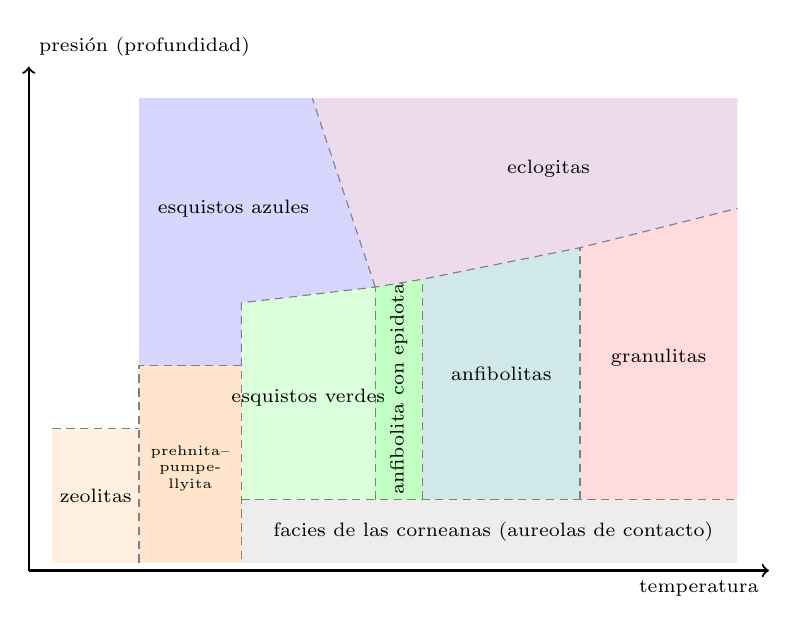
\begin{tikzpicture}[font=\scriptsize, x=1cm, y=1cm]
\draw[->, thick] (0,0) -- (9.4,0) node[below left] {temperatura};
\draw[->, thick] (0,0) -- (0,6.4) node[above right] {presión (profundidad)};
\fill[orange!12] (0.3,0.1) -- (1.4,0.1) -- (1.4,1.8) -- (0.3,1.8) -- cycle;
\fill[orange!20] (1.4,0.1) -- (2.7,0.1) -- (2.7,2.6) -- (1.4,2.6) -- (1.4,1.8) -- cycle;
\fill[green!14] (2.7,0.9) -- (4.4,0.9) -- (4.4,3.6) -- (2.7,3.4) -- cycle;
\fill[green!24] (4.4,0.9) -- (5.0,0.9) -- (5.0,3.7) -- (4.4,3.6) -- cycle;
\fill[teal!18] (5.0,0.9) -- (7.0,0.9) -- (7.0,4.1) -- (5.0,3.7) -- cycle;
\fill[red!14] (7.0,0.9) -- (9.0,0.9) -- (9.0,4.6) -- (7.0,4.1) -- cycle;
\fill[gray!14] (2.7,0.1) -- (9.0,0.1) -- (9.0,0.9) -- (2.7,0.9) -- cycle;
\fill[blue!16] (1.4,2.6) -- (2.7,2.6) -- (2.7,3.4) -- (4.4,3.6) -- (3.6,6.0) -- (1.4,6.0) -- cycle;
\fill[violet!14] (4.4,3.6) -- (5.0,3.7) -- (7.0,4.1) -- (9.0,4.6) -- (9.0,6.0) -- (3.6,6.0) -- cycle;
\draw[gray, densely dashed] (1.4,0.1) -- (1.4,2.6) -- (2.7,2.6) -- (2.7,0.1);
\draw[gray, densely dashed] (0.3,1.8) -- (1.4,1.8);
\draw[gray, densely dashed] (2.7,0.9) -- (9.0,0.9);
\draw[gray, densely dashed] (4.4,0.9) -- (4.4,3.6) (5.0,0.9) -- (5.0,3.7) (7.0,0.9) -- (7.0,4.1);
\draw[gray, densely dashed] (2.7,2.6) -- (2.7,3.4) -- (4.4,3.6) -- (5.0,3.7) -- (7.0,4.1) -- (9.0,4.6);
\draw[gray, densely dashed] (4.4,3.6) -- (3.6,6.0);
\node at (0.85,0.95) {zeolitas};
\node[align=center, font=\tiny] at (2.05,1.3) {prehnita--\\pumpe-\\llyita};
\node at (3.55,2.2) {esquistos verdes};
\node[rotate=90] at (4.7,2.3) {anfibolita con epidota};
\node at (6.0,2.5) {anfibolitas};
\node at (8.0,2.7) {granulitas};
\node at (5.9,0.5) {facies de las corneanas (aureolas de contacto)};
\node at (2.6,4.6) {esquistos azules};
\node at (6.6,5.1) {eclogitas};
\end{tikzpicture}
\par\smallskip{\small La \omterm{def:b2:metamorphic-facies:facies}{red de facies}, esquemática: el orden de las facies de la tabla en
el plano presión--temperatura. Las fronteras son graduales y se dibujan sin números a
propósito: las facies se definen por asociaciones, y las reacciones que las delimitan dependen
de la composición de cada roca.}
\end{omfigure}
% ledger: scmr:facies, scmr:facies-assemblages

\begin{omfigure}
\centering
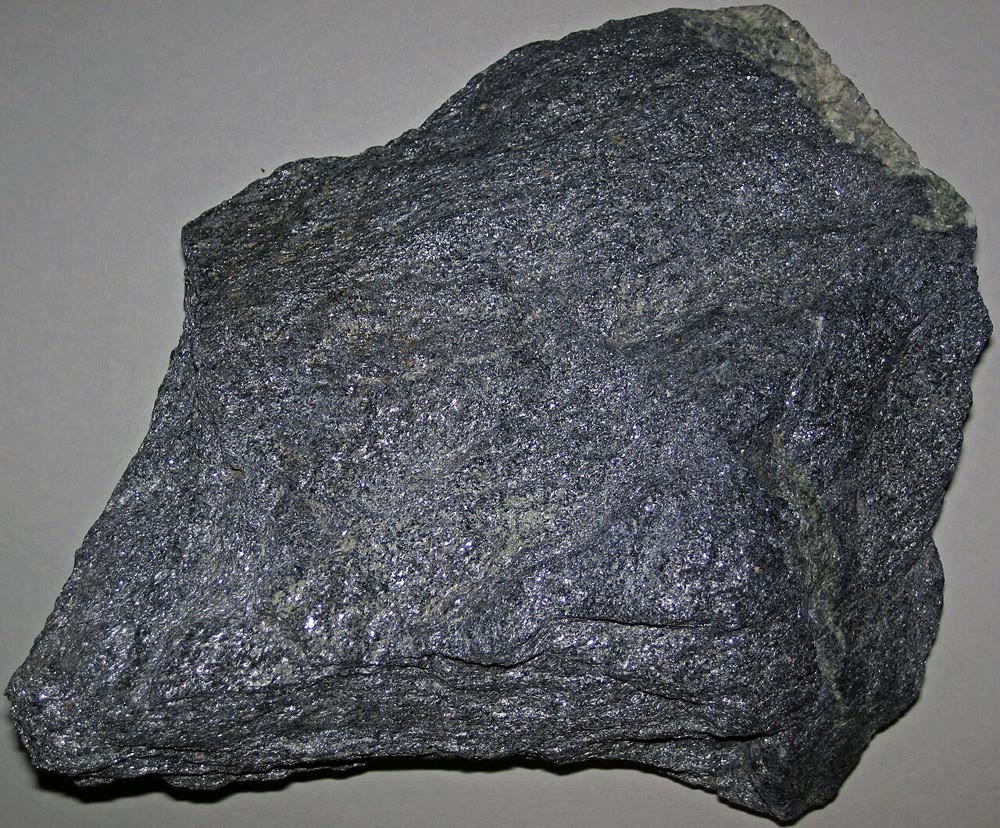
\includegraphics[width=0.27\linewidth]{images/book4/b2-10-blueschist.jpg}\hspace{0.02\linewidth}%
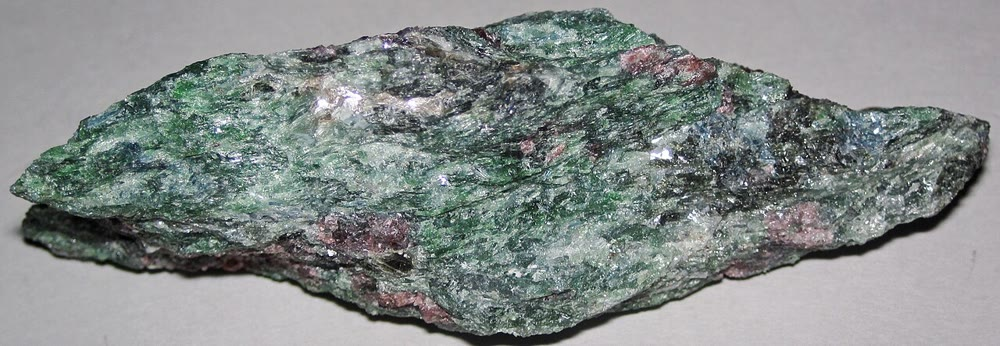
\includegraphics[width=0.69\linewidth]{images/book4/b2-10-eclogite.jpg}
\par\smallskip{\small Dos basaltos metamorfizados. Izquierda: un esquisto azul con lawsonita del
Complejo Franciscano de California, azul por la glaucofana. Derecha: una eclogita del oeste de
Noruega, onfacita verde y granate rojo con algo de cuarzo, cianita y rutilo. Fotografías de
James St.~John, CC BY 2.0.}
\end{omfigure}

Las rocas enterradas y calentadas juntas pasan por las facies en un orden regular, que
refleja la razón entre presión y temperatura a lo largo de su trayectoria: alta en una zona de
subducción, donde se forman los esquistos azules; intermedia en un cinturón de colisión; baja cerca de una intrusión.
El \cref{ch:b2:pt-paths} da nombre a estas series y lee tales trayectorias en los minerales.
% ledger: scmr:facies

\section{El protolito importa}\label{sec:b2:metamorphic-facies:protoliths}

Las facies se definen sobre los basaltos, pero cada \omterm{def:b2:metamorphic-facies:metamorphism}{protolito} registra las mismas condiciones en
sus propios minerales.

\begin{definition}[Metapelita; metabasita]\label{def:b2:metamorphic-facies:protoliths}
Una \emph{metapelita}\index{metapelita} es una lutita (una pelita) metamorfizada, rica en
aluminio y potasio, cuyas asociaciones contienen micas, clorita, granate, estaurolita y
los aluminosilicatos. Una \emph{metabasita}\index{metabasita} es un basalto, un
gabro u otra roca máfica metamorfizados, ricos en calcio, magnesio y hierro, cuyas asociaciones definen
las facies.
\end{definition}

En una \omterm{def:b2:metamorphic-facies:protoliths}{metapelita} los minerales índice del volumen de bachillerato aparecen sucesivamente a medida que
aumenta el grado (clorita, biotita, granate, estaurolita, cianita, sillimanita), la
reacción moscovita + cuarzo de este capítulo forma sillimanita y feldespato potásico a temperatura
aún más alta, y el aluminosilicato presente indica de qué lado del punto
triple pasó la roca. Una caliza o una dolomía metamorfizada se convierte en un mármol, de calcita o de
dolomita; los carbonatos impuros, con sílice y arcilla, se convierten en rocas calcosilicatadas cuyas
reacciones de descarbonatación liberan dióxido de carbono; una arenisca cuarzosa se convierte en una cuarcita,
que apenas muestra otra cosa que su tamaño de grano. Una \omterm{def:b2:metamorphic-facies:protoliths}{metapelita} de la zona de la clorita y un
metabasalto a su lado, a la misma presión y temperatura, no se parecen en nada: el
segundo es una roca verde de actinolita, clorita, epidota y albita. Un solo conjunto de condiciones,
dos asociaciones.
% ledger: iugs:barrow, day73:ms-qz, scmr:facies-assemblages

\section{Ejercicios}

\begin{exercise}[$\star$]\label{exo:b2:metamorphic-facies:1}
Nómbrese el tipo de \omterm{def:b2:metamorphic-facies:metamorphism}{metamorfismo}: (a) una caliza recristalizada en mármol a menos de
\qty{500}{m} de un granito; (b) una roca de grano fino, bandeada, a lo largo de una gran falla
de desgarre, con los granos triturados y recristalizados; (c) un basalto de la corteza oceánica cuyo
vidrio se ha transformado en clorita y zeolitas cerca de una dorsal, con sus minerales solo parcialmente
reemplazados; (d) areniscas volcánicas en la base de una pila de \qty{10}{km} de espesor,
recristalizadas sin esquistosidad.
\end{exercise}
% ledger: scmr:types

\begin{exercise}[$\star$]\label{exo:b2:metamorphic-facies:2}
A partir de la tabla de los aluminosilicatos, calcúlense $\Delta_r S$, $\Delta_r V$ y la
\omterm{def:b2:metamorphic-facies:clapeyron}{pendiente de Clapeyron} de cianita $\to$ sillimanita, en \unit{bar/K} y en \unit{MPa/K}. ¿Cuánto
cambia la presión de equilibrio en \qty{100}{\celsius}?
\end{exercise}
% ledger: rh95:al2sio5

\begin{exercise}[$\star$]\label{exo:b2:metamorphic-facies:3}
¿A qué facies pertenece cada metabasalto? (a) actinolita, albita, clorita y
epidota; (b) glaucofana y lawsonita; (c) hornblenda y plagioclasa con un
\qty{30}{\percent} de anortita; (d) onfacita y granate, sin plagioclasa.
\end{exercise}
% ledger: scmr:facies-assemblages

\begin{exercise}[$\star$]\label{exo:b2:metamorphic-facies:4}
(a) A partir de la masa molar \qty{162.046}{g.mol^{-1}} y de los volúmenes molares 44.15, 51.52 y
\qty{49.86}{cm^3.mol^{-1}}, calcúlense las densidades de la cianita, la andalucita y la sillimanita.
(b) ¿Cuál favorece la presión, y por qué? (c) Las bases de datos mineralógicas dan 3.61, 3.15 y
\qty{3.24}{g.cm^{-3}}: ¿por qué pueden diferir los cristales naturales de las fases puras?
\end{exercise}
% ledger: rh95:al2sio5, webmineral:polymorphs

\begin{exercise}[$\star\star$]\label{exo:b2:metamorphic-facies:5}
Para cianita $\to$ andalucita, $\Delta_r H = \qty{3.9}{kJ}$, $\Delta_r S =
\qty{8.59}{J.K^{-1}}$, $\Delta_r V = \qty{0.737}{J.bar^{-1}}$. (a) ¿Qué polimorfo es
estable a \qty{25}{\celsius} y \qty{1}{bar}? (b) ¿A qué temperatura coexisten ambos
a \qty{1}{bar}? (c) Calcúlese la presión de equilibrio a \qty{400}{\celsius} y
compárese con los \qty{2.54}{kbar} experimentales. (d) ¿Por qué se encuentra sin embargo andalucita
en rocas que se enfriaron hasta la superficie?
\end{exercise}
% ledger: rh95:al2sio5, hm93:table11

\begin{exercise}[$\star\star$]\label{exo:b2:metamorphic-facies:6}
Póngase a prueba el paso (2) del método. A \qty{1000}{K} las tablas dan $S_T$ = 285.02 para la cianita
y 296.44 para la sillimanita, y $(H_T - H_{298})/T$ = 122.29 y 121.39
(\unit{J.mol^{-1}.K^{-1}}). (a) Calcúlense $\Delta_r H$, $\Delta_r S$ y $\Delta_r G$ de
cianita $\to$ sillimanita a \qty{1000}{K} y \qty{1}{bar}. (b) Compárense con los valores
constantes de la tabla. (c) ¿Qué polimorfo es estable allí, y qué tamaño tiene el error del
método simple?
\end{exercise}
% ledger: rh95:al2sio5-ht, rh95:al2sio5

\begin{exercise}[$\star\star$]\label{exo:b2:metamorphic-facies:7}
La calcita y el aragonito (\ce{CaCO3}) tienen, a \qty{298.15}{K}, $\Delta_f G$ = $-1128.5$ y
$-1127.4$ \unit{kJ.mol^{-1}}, $S$ = 91.7 y 88.0 \unit{J.mol^{-1}.K^{-1}}, $V$ = 36.93
y \qty{34.15}{cm^3.mol^{-1}}, y entalpías de formación iguales. (a) Hállese la
presión de equilibrio a \qty{25}{\celsius}. (b) Calcúlese la \omterm{def:b2:metamorphic-facies:clapeyron}{pendiente de Clapeyron}. (c) Hállese la
presión de equilibrio a \qty{300}{\celsius}. (d) Muchas conchas son de aragonito y
viven a \qty{1}{bar}: ¿qué indica eso?
\end{exercise}
% ledger: rh95:cc-ar

\begin{exercise}[$\star\star$]\label{exo:b2:metamorphic-facies:8}
Para albita $\to$ jadeíta + cuarzo, las tablas dan $\Delta_r H = \qty{-5.0}{kJ}$,
$\Delta_r S = \qty{-32.4}{J.K^{-1}}$, $\Delta_r V = \qty{-1.698}{J.bar^{-1}}$. (a)
Calcúlese la \omterm{def:b2:metamorphic-facies:clapeyron}{pendiente de Clapeyron}. (b) Calcúlese la presión de equilibrio a \qty{500}{\celsius}.
(c) Las entalpías de formación de la albita, la jadeíta y el cuarzo tienen incertidumbres de 2.6, 3.6
y \qty{1.0}{kJ.mol^{-1}}; combinándolas como errores independientes, ¿qué incertidumbre tiene esa
presión? (d) ¿Por qué carece de plagioclasa la facies de las eclogitas?
\end{exercise}
% ledger: rh95:ab-jd-qz, scmr:facies-assemblages

\begin{exercise}[$\star\star$]\label{exo:b2:metamorphic-facies:9}
La moscovita + cuarzo se descompone a 603, 637 y \qty{662}{\celsius} a 1, 2 y
\qty{3}{kbar}. (a) Calcúlese la pendiente de la línea entre cada par de puntos. (b) Si la
entropía de reacción apenas cambia en este intervalo, ¿en qué factor disminuyó $\Delta_r V$
del primer intervalo al segundo? (c) ¿Qué fase es responsable?
\end{exercise}
% ledger: day73:ms-qz

\begin{exercise}[$\star\star\star$]\label{exo:b2:metamorphic-facies:10}
Con las propiedades constantes del método: (a) calcúlense las presiones de las tres
reacciones a \qty{600}{\celsius}; (b) demuéstrese que a \qty{600}{\celsius} y a la presión de
cianita $=$ andalucita, la sillimanita es el polimorfo más estable, de modo que ese punto de
la línea es metaestable; (c) ¿qué polimorfo es estable a \qty{600}{\celsius} y
\qty{4}{kbar}, y a \qty{600}{\celsius} y \qty{7}{kbar}?
\end{exercise}
% ledger: rh95:al2sio5

\begin{exercise}[$\star\star\star$]\label{exo:b2:metamorphic-facies:11}
Un esquisto contiene juntas cianita, andalucita y sillimanita, las tres crecidas en
equilibrio. (a) Con el punto triple experimental, $504 \pm \qty{20}{\celsius}$ y
$3.75 \pm \qty{0.25}{kbar}$, y una corteza de densidad \qty{2700}{kg.m^{-3}} ($g =
\qty{9.81}{m.s^{-2}}$), ¿a qué profundidad creció? (b) Tomando \qty{10}{\celsius} en la
superficie, ¿qué gradiente térmico medio implica? (c) ¿Por qué son raras esas rocas?
\end{exercise}
% ledger: hm93:triple

\begin{exercise}[$\star\star\star$]\label{exo:b2:metamorphic-facies:12}
Dos rocas se entierran hasta la profundidad $z$, desde \qty{10}{\celsius} en la superficie: la roca X a lo largo de
\qty{10}{\celsius.km^{-1}} hasta \qty{30}{km} bajo rocas de densidad media
\qty{3000}{kg.m^{-3}}, la roca Y a lo largo de \qty{30}{\celsius.km^{-1}} hasta \qty{20}{km} bajo rocas
de densidad media \qty{2800}{kg.m^{-3}}. (a) Calcúlense $T$ y $P$ al final de cada trayectoria.
(b) Con las líneas de propiedades constantes (calcita $=$ aragonito: $P = 13.31\,T$ bar con $T$
en kelvin; albita $=$ jadeíta + cuarzo del \cref{exo:b2:metamorphic-facies:8}; los aluminosilicatos de la
tabla), ¿contiene cada roca aragonito o calcita, jadeíta + cuarzo o albita, y qué
aluminosilicato contiene? (c) ¿Cuál es la trayectoria más fría, de alta presión, y en qué facies termina cada una?
\end{exercise}
% ledger: rh95:cc-ar, rh95:ab-jd-qz, rh95:al2sio5

\section{Problema: construir el punto triple}

\begin{problem}[{Problema de fin de semana --- el diagrama de los aluminosilicatos a partir de las tablas, y hasta
qué punto fiarse de él}]
\label{pb:b2:metamorphic-facies:1}
Úsense la tabla de los aluminosilicatos (\qty{298.15}{K}, \qty{1}{bar}) y el método de
este capítulo, con $\Delta_r H$, $\Delta_r S$ y $\Delta_r V$ constantes; escríbase $T$ en
kelvin y $P$ en bar, y despréciese el 1 de $P - 1$.

\noindent\textbf{Parte I --- Las reacciones.}
\begin{enumerate}
\item Calcúlense $\Delta_r H$, $\Delta_r S$ y $\Delta_r V$ para cianita $\to$ andalucita.
\item Hágase lo mismo para cianita $\to$ sillimanita.
\item Hágase lo mismo para andalucita $\to$ sillimanita, y compruébese que cada propiedad es la
diferencia de las dos primeras.
\item ¿Qué polimorfo tiene la mayor entropía, cuál el menor volumen? ¿De qué lado
de cada línea quedará cada uno?
\item Calcúlense las tres \omterm{def:b2:metamorphic-facies:clapeyron}{pendientes de Clapeyron}.
\item ¿Por qué es negativa la pendiente de andalucita $\to$ sillimanita?
\end{enumerate}

\noindent\textbf{Parte II --- Por dónde van las líneas.}
\begin{enumerate}[resume]
\item Calcúlese $\Delta_r G$ de las dos primeras reacciones a \qty{298.15}{K}. ¿Qué
polimorfo es estable en la superficie?
\item ¿A qué temperatura (en \unit{\celsius}) alcanza cada reacción el equilibrio a
\qty{1}{bar}?
\item De las tres temperaturas de la pregunta~8, ¿cuáles son equilibrios estables y cuáles
metaestables? (Úsese el orden de las tres a \qty{1}{bar}.)
\item Calcúlese la presión de cianita $=$ andalucita a \qty{400}{\celsius}; los
experimentos dan \qty{2.54}{kbar}.
\item Calcúlese la presión de cianita $=$ sillimanita a \qty{700}{\celsius}; los
experimentos dan \qty{7.86}{kbar}.
\item Esbócense las tres líneas entre 200 y \qty{900}{\celsius}.
\end{enumerate}

\noindent\textbf{Parte III --- El punto triple.}
\begin{enumerate}[resume]
\item Escríbanse las dos primeras líneas como $P = a_i T - b_i$; dense $a_1$, $b_1$, $a_2$, $b_2$.
\item Despéjese la temperatura de su intersección.
\item Calcúlese su presión.
\item Compruébese que andalucita $=$ sillimanita pasa por ella.
\item Compárese con los valores experimentales $504 \pm \qty{20}{\celsius}$ y $3.75 \pm
\qty{0.25}{kbar}$.
\item Con la dependencia de la temperatura de las tablas, el punto triple se desplaza a
\qty{536}{\celsius} y \qty{4.20}{kbar}. ¿Lo acercó el refinamiento a los
experimentos? ¿Qué sugiere eso sobre la principal fuente de error?
\end{enumerate}

\noindent\textbf{Parte IV --- Hasta qué punto fiarse.}
\begin{enumerate}[resume]
\item Auméntese en \qty{1}{kJ} la entalpía de formación de la andalucita. ¿Cuánto se desplaza
en presión la línea cianita $=$ andalucita, a temperatura fija?
\item ¿Cuánto se desplaza en temperatura el punto triple?
\item Hágase lo mismo para un aumento de \qty{1}{kJ} en la entalpía de la sillimanita.
\item Cada entalpía tiene una incertidumbre de \qty{2.0}{kJ}. ¿Qué intervalo de temperaturas del punto
triple permiten los datos calorimétricos por sí solos?
\item ¿Cómo pueden entonces las tablas termodinámicas reproducir el diagrama experimental con un margen de
\qty{30}{\celsius}?
\item Dese la temperatura del punto triple calculada en la Parte III, redondeada al
grado: el número clave de este problema.
\end{enumerate}
\end{problem}
% ledger: rh95:al2sio5, rh95:al2sio5-ht, hm93:triple, hm93:table11, hm93:adjusted
